% !TEX program = xelatex
\documentclass[a4paper]{article}
\usepackage{amsmath}
\usepackage{amsthm}
\usepackage[left=1.8cm,right=1.8cm,top=2.2cm,bottom=2.0cm]{geometry}
\usepackage{ctex}
\usepackage{enumerate}
\usepackage{fancyhdr}
\usepackage{xpatch}
\usepackage{graphicx} 
\usepackage{float} 
\usepackage{subfigure} 
\usepackage{amsfonts}
\usepackage{mathtools}
\usepackage{framed}
\usepackage{multicol}
\usepackage{listings}
\usepackage{hyperref}
\usepackage{tikz}
\usetikzlibrary{automata,positioning}
\theoremstyle{definition}
\newtheorem*{solution*}{\textbf{Solution:}}
\newtheorem*{proof*}{\textbf{Proof:}}
\newtheorem{theorem}{Theorem}[subsection]
\newtheorem{definition}{Definition}[subsection]
\newtheorem{lemma}{Lemma}[subsection]
\makeatletter

\AtBeginDocument{\xpatchcmd{\@thm}{\thm@headpunct{.}}{\thm@headpunct{}}{}{}}
\makeatother

\pagestyle{fancy}
\renewcommand{\baselinestretch}{1.15}

\usepackage{paralist}
\let\itemize\compactitem
\let\enditemize\endcompactitem
\let\enumerate\compactenum
\let\endenumerate\endcompactenum
\let\description\compactdesc
\let\enddescription\endcompactdesc

% shorten footnote rule
\xpatchcmd\footnoterule
  {.4\columnwidth}
  {1in}
  {}{\fail}

\title{CS 131 Compilers: Discussion 8: Intermediate Representations: Basic Block and CFG \& Mid Term Preparation2}
\author{\textbf{杨易为}~~\textbf{季杨彪}~~\textbf{尤存翰} \\ \texttt{ \{yangyw,jiyb,youch\}@shanghaitech.edu.cn}}


\begin{document}
\maketitle
\section{Intermediate Representations}
An Intermediate Representation (IR) is an intermediate (neither source nor target) form of a program. There are various types of IRs:
\begin{enumerate}
  \item Section
  \begin{enumerate}
    \item \textbf{Abstract Syntax Trees} (AST): a simplified Parse Tree.\\
    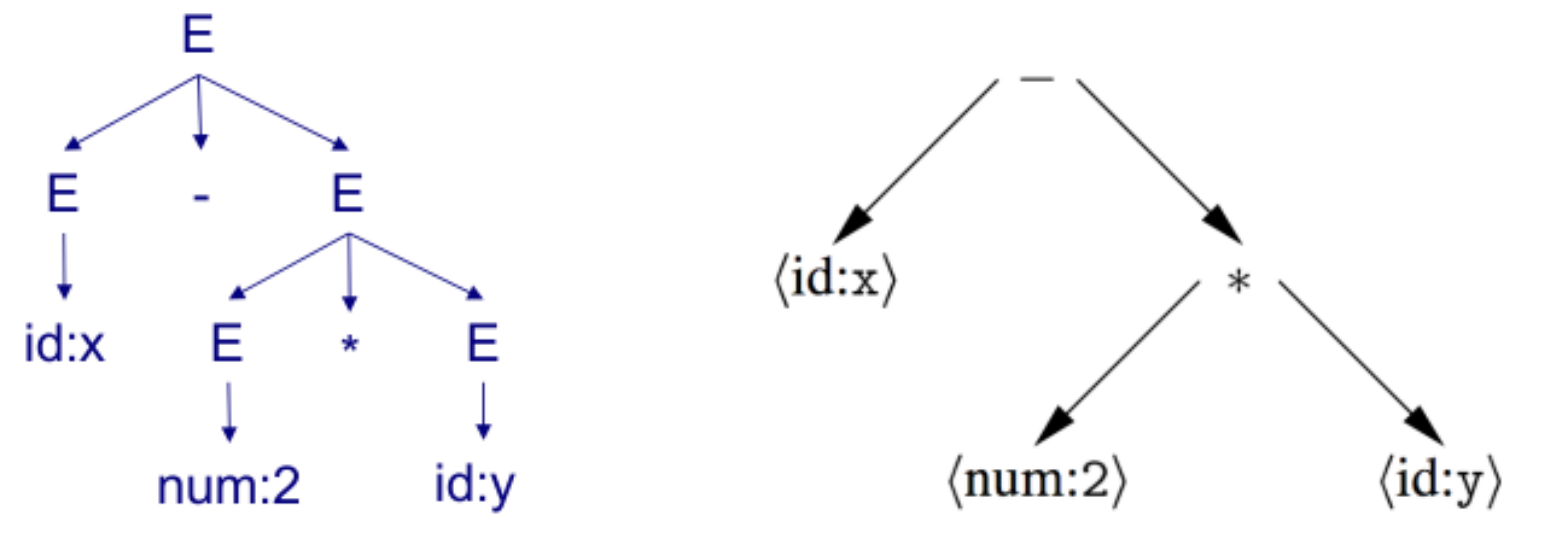
\includegraphics[width=10cm]{img/Snipaste_2021-04-19_07-08-30.png}
    \begin{itemize}
      \item + close to source compactdesc
      \item + suitable for source-source translation
      \item - Traversal \& Transformations are expensive
      \item - Pointer-intensive
      \item - Memory-allocation-intensive
    \end{itemize}

    \item \textbf{Directed Acyclic Graphs} (DAG): DAG is an optimized AST, with identical nodes \textit{shared}.\\
    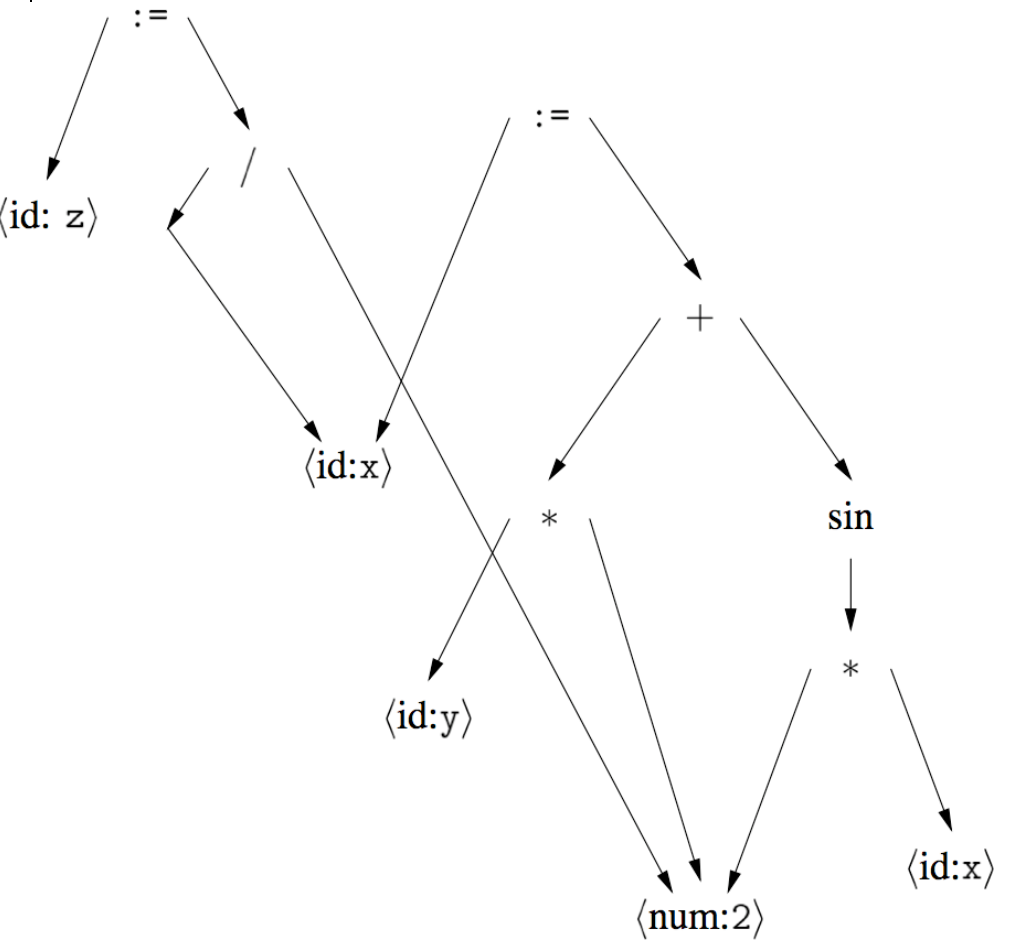
\includegraphics[width=10cm]{img/Snipaste_2021-04-19_07-11-03.png}
    \begin{itemize}
      \item + Explicit sharing
      \item + Exposes redundancy, more efficient, useful for dynamic pipelining analysis
      \item - Difficult to transform
      \item - Analysis usage Practical usage
    \end{itemize}
    \item \textbf{Control Flow Graphs} (CFG): CFG is a flow chart of program execution. Is a conservative approximation of the Control Flow, because only one branch will be actually executed.\\
    A Basic Block is a consecutive sequence of Statements $S_{1}, \ldots, S_{n}$, where flow must enter this block only at $S_{1}$, AND if $S_{1}$ is executed, then $S_{2}, \ldots, S_{n}$ are executed strictly in that order, unless one Statement causes halting.

    \begin{itemize}
      \item The Leader is the first Statement of a Basic Block
      \item A Maximal Basic Block is a maximal-length Basic Block
    \end{itemize}
Nodes of a CFG are Maximal Basic Blocks, and Edges of a CFG represent control flows
$\exists$ edge $b_{1} \rightarrow b_{2}$ iff control may transfer from the last Statement of $b_{1}$ to the first Statement of $b_{2}$
    \item \textbf{Data Dependence Graphs} (DDG):
  \end{enumerate}
\end{enumerate}
\begin{center}
  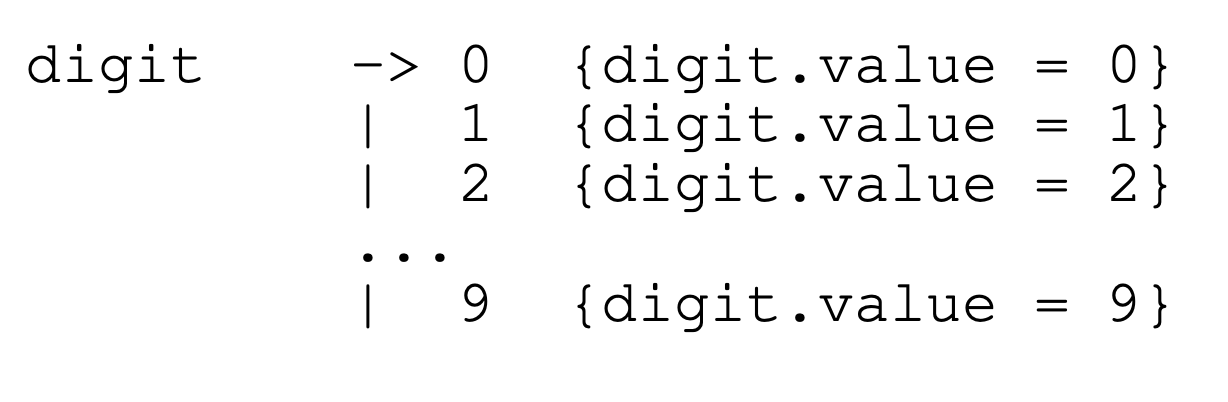
\includegraphics[height=3cm]{img/Snipaste_2021-04-12_17-41-51.png}
  \end{center}
  Attributes may be passed up a parse tree to be used by other productions:
  
  \begin{center}
    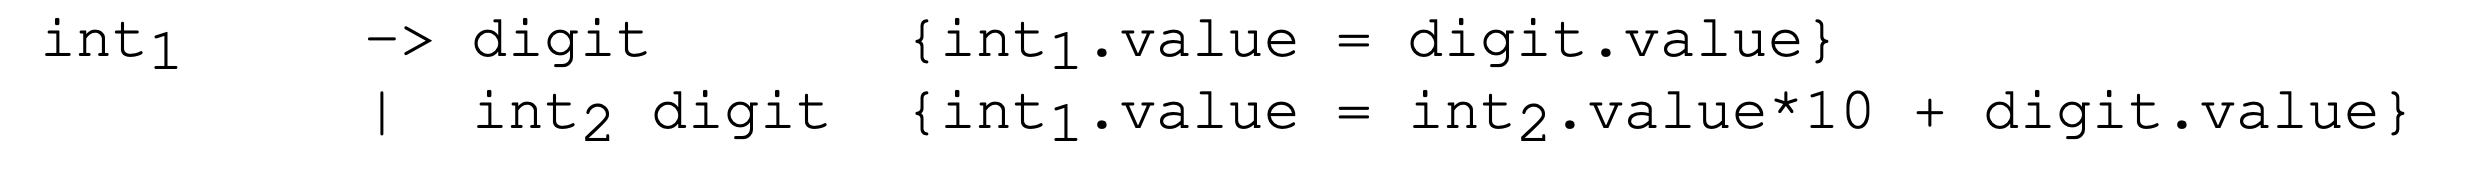
\includegraphics[height=1.2cm]{img/Snipaste_2021-04-12_17-42-34.png}
    \end{center}
    
    There are two types of attributes we might encounter: synthesized or inherited. Synthesized attributes are those attributes that are passed up a parse tree, i.e., the left-
    side attribute is computed from the right-side attributes. The lexical analyzer usually supplies the attributes of terminals and the synthesized ones are built up for the nonterminals and passed up the tree.
    
    \begin{center}
      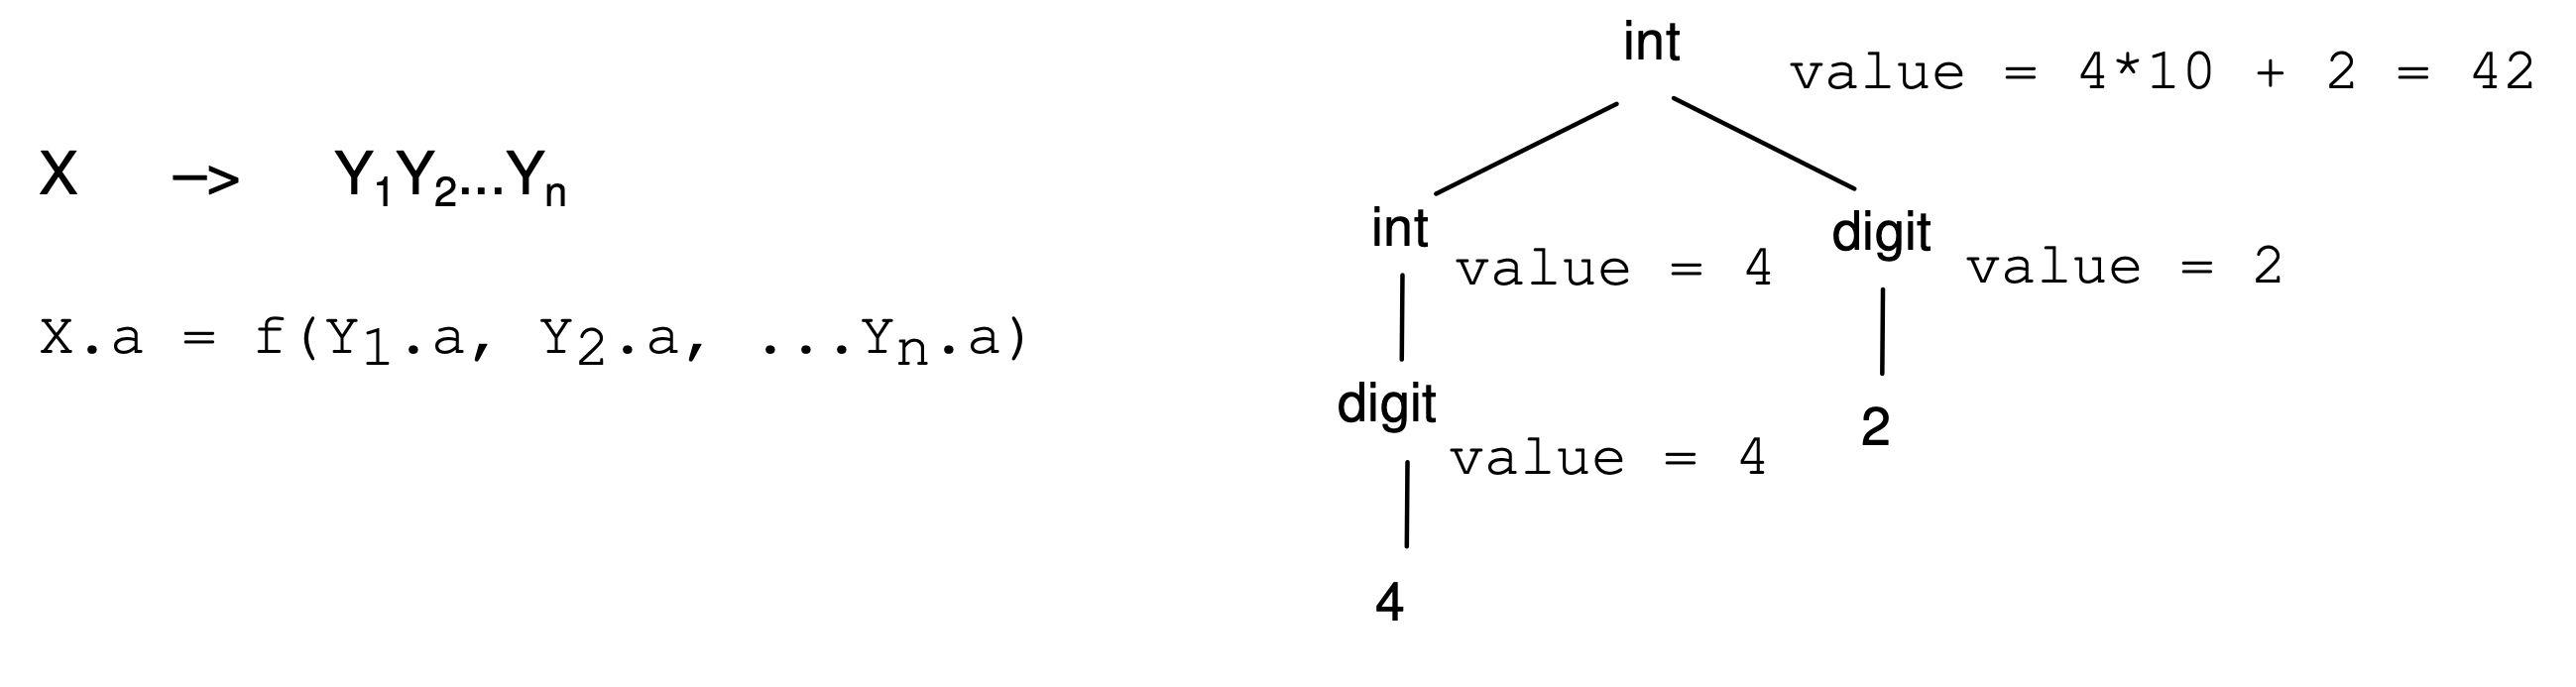
\includegraphics[height=3cm]{img/Snipaste_2021-04-12_17-43-29.png}
      \end{center}
      
      Inherited attributes are those that are passed down a parse tree, i.e., the right-side attributes are derived from the left-side attributes (or other right-side attributes). These attributes are used for passing information about the context to nodes further down the tree.
      \begin{center}
        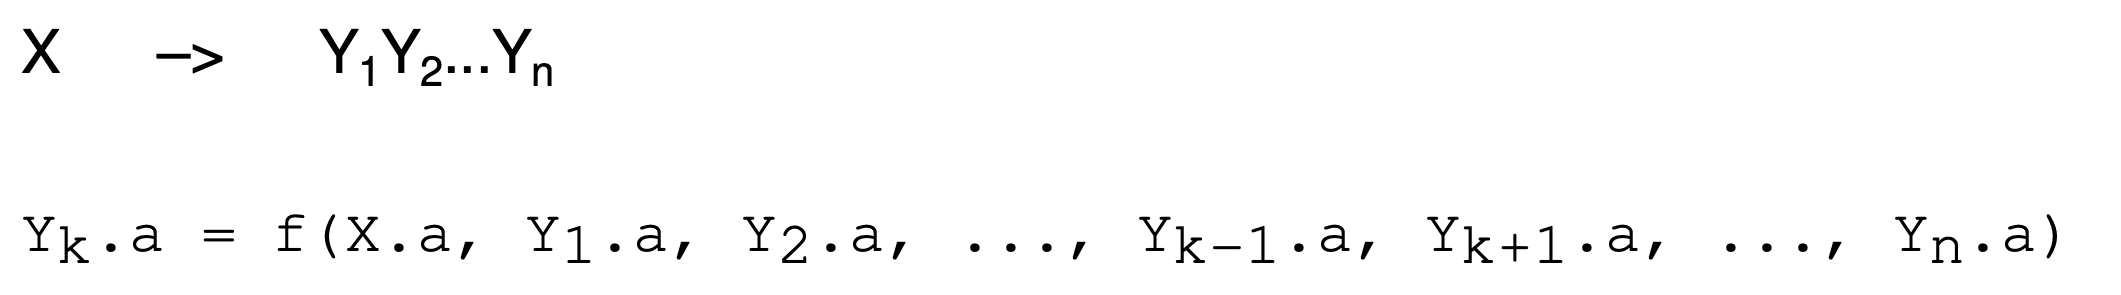
\includegraphics[height=1.5cm]{img/Snipaste_2021-04-12_17-44-09.png}
        \end{center}
Bison is a little bit different, which is bigger than LALR(k).


\section{Mid Term preparation}
\subsection{Regular Expressions}
\begin{enumerate}
   \item Write a regex that matches binary strings divisible by 8.
   \item Provide aregulargrammar for the regex from part (a).
 \end{enumerate}

  \subsection{Finite State Automata}
  \begin{enumerate}
    \item Write the corresponding NFA for the regular expression $(0|1)?(10|01)+$;
    \item Convert the NFA from part (a) into a DFA.
  \end{enumerate}
  
  \subsection{Grammar Rewriting and LL(k) Parsing}
  $$
\begin{aligned}
&\begin{aligned}
S &: E \dashv \\
E: & E+E \\
& \mid E * E
\end{aligned}\\
&\quad 
 \ \mid \text { ID }
\end{aligned}
$$
  \begin{enumerate}
    \item Show that the grammar is ambiguous with two different leftmost derivations of the string $a+b*c$;
    \item Rewrite this grammar so that it preserves the standard order of operations, is LL(1),and is unambiguous.  Draw the resulting tree for the string $a+b*c$;
    \item Write down the equivalent unambiguous grammar that enforces both left associativity and correct precedence.  Why can’t this be achieved with an LL(1) grammar?
  \end{enumerate}

  \subsection{Earley’s Algorithm}

  \begin{center}
    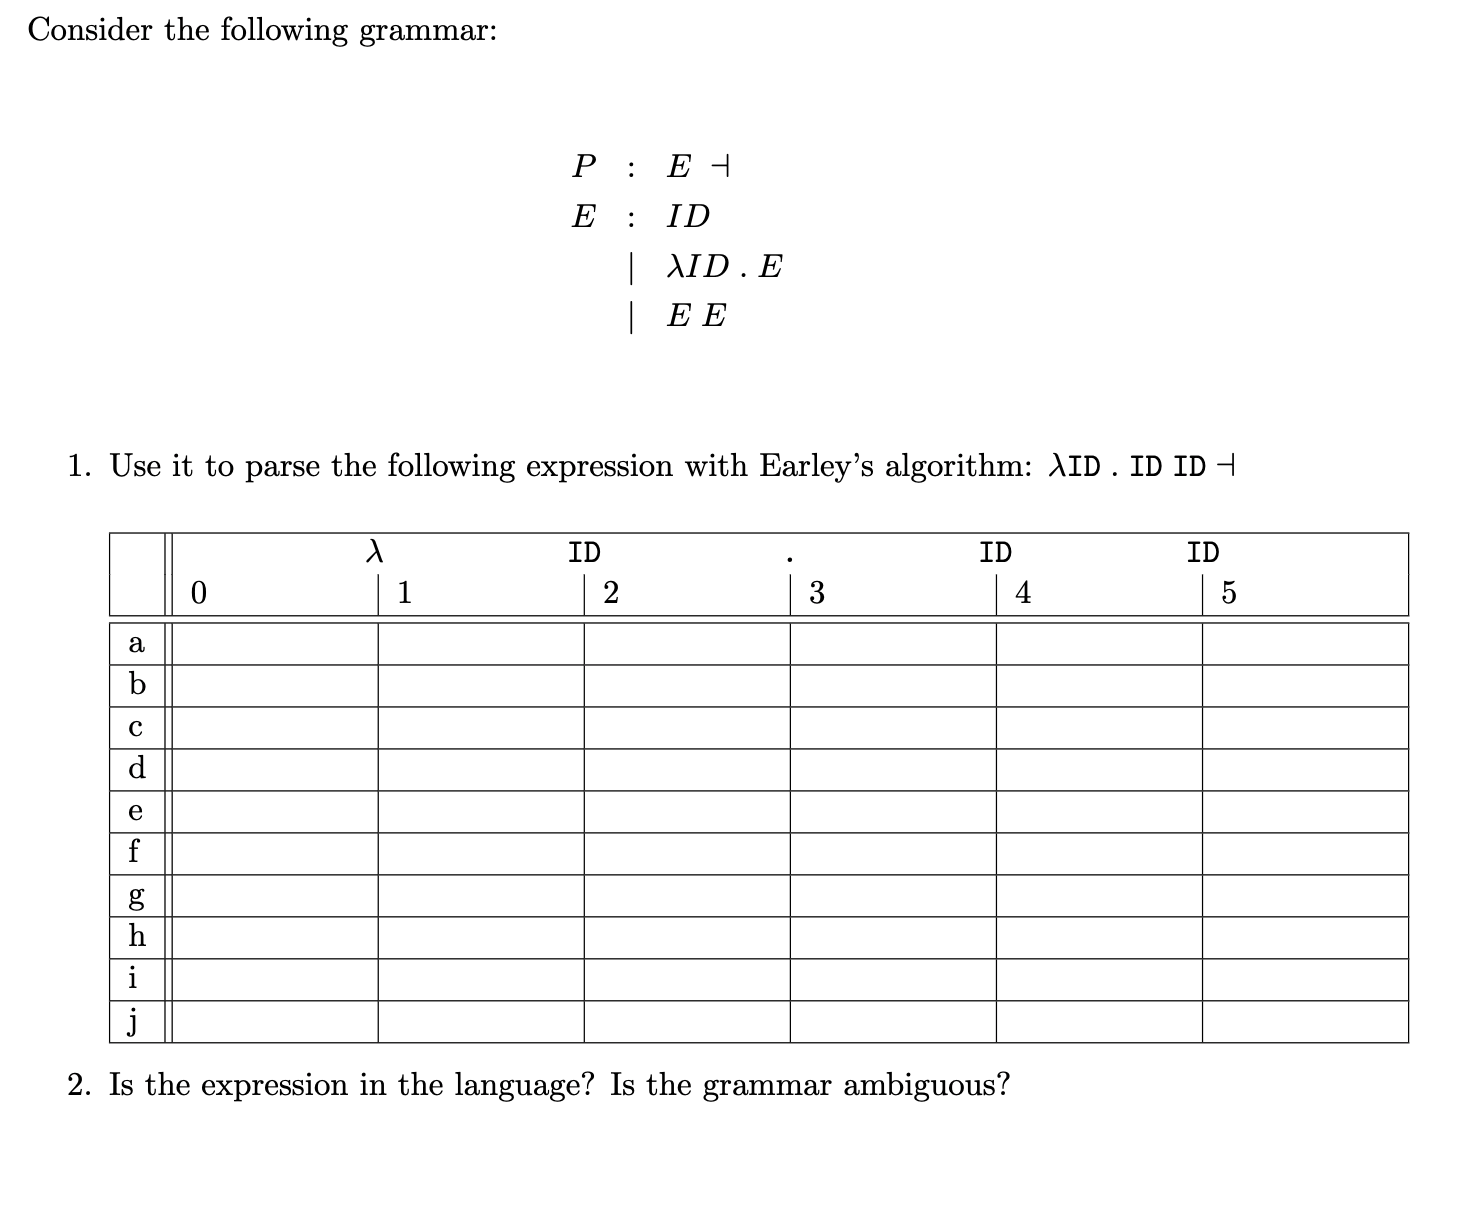
\includegraphics[height=12cm]{img/Snipaste_2021-04-12_17-39-39.png}
    \end{center}
    
\end{document}
